
\documentclass[10pt,stdletter,dateno,sigleft]{newlfm}
\usepackage{pdfpages}
\usepackage{charter} % Use the Charter font for the document text

\newsavebox{\Luiuc}\sbox{\Luiuc}{\parbox[b]{1.75in}{\vspace{0.5in}
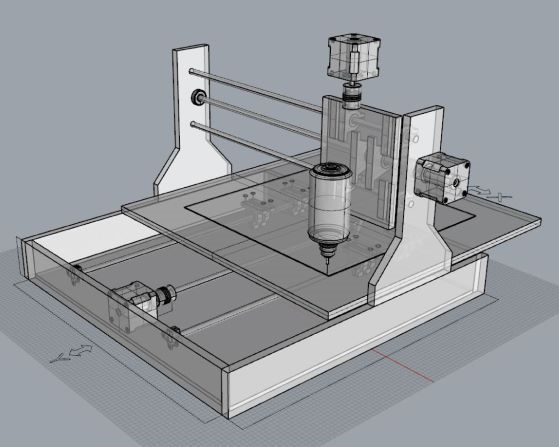
\includegraphics[width=1.2\linewidth]{CNC.PNG}}} % LOGOTIPO DE LA EMPRESA EN LA PARTE SUPERIOR IZQUIERDA
\makeletterhead{Uiuc}{\Lheader{\usebox{\Luiuc}}}

\newlfmP{sigsize=50pt} % DISMINULLE EL CAMPO DE FIRMA

\lthUiuc % MUESTRA EL LOGO DE LA CNC logo

%----------------------------------------------------------------------------------------
%	YOUR NAME AND CONTACT INFORMATION
%----------------------------------------------------------------------------------------

\namefrom{Everardo Estrella} % Name

\addrfrom{
\date\\[08 de Octubre del 2019] % Date
 \\ % Address
Proyecto CNC
}

%----------------------------------------------------------------------------------------
%	ADDRESSEE AND GREETING/CLOSING
%----------------------------------------------------------------------------------------

\greetto{Desarrollo de un Robot serial CNC} 
\closeline{A continuacion se adjunta los planos del Robot serial CNC y desarrollo de construccion}

\nameto{Everardo Estrella} 

\addrto{
Ingeneria en Mecatronica \\ 
Universidad Politecnica \\
Proyecto Final \\
Cinematica de Robots
}

%----------------------------------------------------------------------------------------

\begin{document}
\date{FECHA 2019}
\begin{newlfm}

%----------------------------------------------------------------------------------------
%	LETTER CONTENT
%----------------------------------------------------------------------------------------

\includepdf[pages=-]{F3}
Definicion de Materia: La cinemática de robots La cinemática de un robot es el estudio de los movimientos de un robot. En un análisis cinemático la posición, velocidad y aceleración de cada uno de los elementos del robot son calculados sin considerar las fuerzas que causan el movimiento. La relación entre el movimiento y las fuerzas asociadas son estudiadas en la dinámica de robots.

Propósito de Materia: El propósito de esta materia es el conocimiento de los tipos de robots industriales donde se pide la elaboración de un robot serial como proyecto a realizar para el período séptimo cuatrimestre, y la elaboración del robot serial CNC. 
 
%----------------------------------------------------------------------------------------

\end{newlfm}

\end{document}